% Supplemental direction tips on the user's unchanged vector drawing.
% Coordinates are PDF points from the panel's upper-left corner.
\documentclass[border=0pt]{standalone}
\usepackage{graphicx,tikz}
\usetikzlibrary{arrows.meta}
\definecolor{acol}{RGB}{245,154,35}
\definecolor{dcol}{RGB}{130,33,139}
\begin{document}%
\begin{tikzpicture}[x=1bp,y=-1bp,
  tip/.style={line width=.55bp,-{Stealth[length=3.7bp,width=2.7bp]},line cap=round},
  atip/.style={tip,acol},dtip/.style={tip,dcol}]
\path[use as bounding box] (0,0) rectangle (278,292);
\begin{scope}[overlay]
\node[anchor=north west,inner sep=0pt,outer sep=0pt] at (0,0)
  {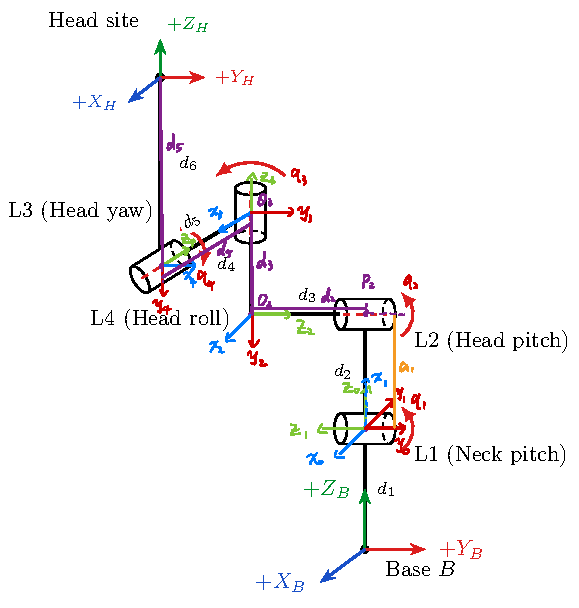
\includegraphics[width=278bp,height=292bp]{../assets/dh_head_handdrawn.pdf}};
% a_1: the orange neck-to-head-pitch dimension, upward.
\draw[atip] (189.6,158.8)--(189.6,151.0);
% d_2: head-pitch intermediate point to its selected origin, leftward.
\draw[dtip] (128.9,148.1)--(121.1,148.1);
% d_3: head-pitch origin to head-yaw origin, upward.
\draw[dtip] (120.6,110.2)--(120.6,102.5);
% d_4: existing purple offset segment, down-left toward head roll.
\draw[dtip] (85.0,128.5)--(78.1,132.5);
% d_5: the existing head-roll-to-site component, upward.
\draw[dtip] (77.0,45.4)--(77.0,37.6);
\end{scope}
\end{tikzpicture}%
\end{document}
